\section{Datenmodelle zur Effizienzberechnung}
Die Basis für eine jede Optimierung ist es Kennzahlen zu ermitteln die es ermöglichen die Effizenz vor und nach der Optimierung zu vergleichen. Das bedeutet, dass der Einsatz von gewissen Mitteln und deren Ertrag gemessen wird. 

In der Literatur werden zwei verschiedene Modellierungsklassen zur Effizenzanalyse empfohlen:\cite{jour:Curtiss2012}\cite{conf:Jian2013}
\begin{itemize}
	\item \textit{Data Envelopment Analysis}, kurz DEA
	\item \textit{Stochastische Frontier Analyse}, kurz SFA
\end{itemize}

\subsection{Data Envelopment Analysis}

DEA ist eine parameterlose Methode um die Effizenz von so genannten \textit{Decision Making Units}, kurz DMUs, zu messen. Eine DMU kann einen oder mehrere Eingaben erwarten und kann auch einen oder mehrere Ausgabewerte besitzen. Um die Effizenz zu messen, wird eine einzige \textit{virtuelle} Eingabe auf eine einzige \textit{virtuelle} Ausgabe abgebildet ohne dabei eine vordefinierte Produktionsfunktion zu erstellen.\cite{jour:Cullinane2006}

Sei $x_k=(x_1k,x_2k,...,x_Mk) \in R^{M}_+$ um die Ausgabewerte $y_k=(y_1k,y_2k,...,y_Nk) \in R^{M}_+$ zu produzieren. Dann bilden die Zeilenvektoren $x_k$ und $y_k$ die Datenmatrizen $X$ bzw. $Y$. Zusätzlich sei $\lambda = (\lambda_1,\lambda_2,...,\lambda_K) \in R^{K}_+$ ein positiver Vektor der die lineare Kombination aus $K$ Firmen. Als letzte zu definierende Größe sei $e = (1,1,...,1)$ ein passend dimensionierter Vektor von Einheitsgrößen.\cite{jour:Cullinane2006}

Das ausgabeorientierte DEA-Modell maximiert die proportionale Steigerung der Ausgabe unter der Bedingung dass der Produktionsraum nicht verlassen wird. Ein ausgabenorientiertes Messproblem kann als eine Reihe von $K$ linearer Programmierungsprobleme abgebildet werden.\cite{jour:Cullinane2006}. Für DEA gibt es mehrere Modelle wie das Verhältnis zu Eingabe/Ausgabe skalieren kann. Zwei häufig verwendete Varianten sind DEA-CCR, nach Charnes, und DEA-BCC, nach Bankes. DEA-CCR beschreibt im Gegensatz zu DEA-BCC Modelle in denen sich Eingabewerte zu Ausgabewerte proportional verändern. Die nötigen \textit{Constraints} für das Lineare Programmieren werden durch beschrieben.

\begin{equation}\label{eq:maxu}
	\begin{tabular}{rr}
		$\underset{U,\lambda}{max}$ & $U$	 	
	\end{tabular}
\end{equation}

\begin{equation}\label{eq:uy}
	\begin{tabular}{rr}
		$Maximiert$ & $U_{y_k}' - Y'\lambda \leqslant 0$	 	
	\end{tabular}
\end{equation}


\begin{equation}\label{eq:xylambda}
	\begin{tabular}{rr}
		$$ & $X_{y_k}'\lambda - x_k' \leqslant 0$	 	
	\end{tabular}
\end{equation}

\begin{equation}\label{eq:lambdagezero}
	\begin{tabular}{rr}
		$$ & $x_k' \geqslant 0$ (DEA-CCR)	 	
	\end{tabular}
\end{equation}

\begin{equation}\label{eq:elambdaequalsone}
	\begin{tabular}{rr}
		$$ & $e\lambda' = 1$ (DEA-BCC)	 	
	\end{tabular}
\end{equation}

Die ausgabeorientierte Messung der technischen Effizenz der k-ten DMU, bezeichnet als $TE_k$, kann so berechnet werden:

\begin{equation}
	TE_k= \frac{1}{U_k}
\end{equation}

Eine weitere Kennzahl die mit DEA-CCR\eqref{eq:lambdagezero} bzw. DEA-BCC\eqref{eq:elambdaequalsone} berechnet werden kann ist die Skalierungseffizenz $SE_k$:

\begin{equation}
	SE_k = \frac{U_{CCR_k}}{U_{BCC_k}}
\end{equation}

In \textit{Cost Efficiency and Farm Self-selection in Precision Farming: The Case of Czech Wheat Production}\cite{jour:Curtiss2012} wird eine zweistufige Berechnung von Effizenzmodellen vorgeschlagen. Dazu wird im ersten Schritt eine DEA durchgeführt. Das resultierende DEA ist definiert als:

\begin{gather}
	min_{\lambda,xic} \; (p'_{i}x_{ci}) \\
	st \;\;\; - y_i+Y\lambda \leq 0, \\
	x_{ci} - X \lambda \leq 0, \\
	\lambda \leq 0.
\end{gather}

Es wird zusätzlich vorgeschlagen, die daraus abgeleitete Betriebseffizenzbewertungen mittels \textit{Endogenous Switching Regression} zu analysieren.

Blancard und Martin weisen in \textit{Energy efficiency measurement in agriculture with imprecise energy content information} darauf hin, dass die Messungen der verbrauten Energie Schwankungen und Unsicherheiten unterworfen ist. Deshalb schlagen sie in der selben Arbeit ein auf DEA basierendes Modell vor, um diese Unsicherheiten bei der Berechnung der Energieeffizenz mit ein zu beziehen um robuste Ergebnise zu erhalten.\cite{jour:Blancard2014}

Der Ansatz basiert darauf, dass eine sg. \textit{Assurance Region}, kurz AR, gefunden wird die eine pessimistische und eine optimistische Grenze fest legt. Diese Grenze wird für jede DMU durch den wünschenswertesten bzw. am wenigsten wünschenswertesten (\textit{least favourable}) errechneten Energieverbrauch (\textit{energy content scenario}) definiert.\cite{jour:Blancard2014}

\subsection{Stochastische Frontier Analysis}
Im Gegensatz zu DEA, nimmt SFA an, dass es eine Funktion mit einem oder mehreren Parametern gibt, die, die Produktionseingabewerte auf die Ausgabewerte abbilden kann. Zusätzlich hat SFA den großen Vorteil, dass die Funktionen so gestaltet werden können, dass nicht nur technische (In-)Effizenz den Ausgabewert beeinflusst sondern auch Ereignisse außerhalb des Einflussbereichs des Produzenten. Dementsprechend besteht der Fehlerterm in SFA aus zwei Komponenten:
\begin{itemize}
	\item Eine einseitige Komponente die, die Effekte von Ineffizenz relative zur stochastischen Marke (\textit{stochastic frontier}) einfängt.
	\item Eine symmetrische Komponente die es erlaubt eine zufällige Variation der Marken (\textit{frontiers}) über Firmen hinweg abzubilden und so die Effekte von Messfehlern, anderem statistischem Rauschen und zufälligen Schocks außerhalb der Firmenkontrolle einzufangen.
\end{itemize}

Daraus folgt, dass eine SFA als Gleichung abgebildet werden kann in der die Effizenz der Firma \textit{k} als $U_k$ bezeichnet wird, wobei $U_k$ positiv sein muss. Die oben angesprochene Komponente, die das statistische Rauschen einfängt, wird als $V_k$ bezeichnet, wobei $V_k$ sowohl negativ wie auch positiv sein kann.\cite{jour:Cullinane2006}

\begin{equation}\label{eq:sfadef}
	y_k = f(x_1k,x_2k,...,x_Mk,U_k,V_k)
\end{equation}

Um solche SFAs zu lösen, muss zu allerst ein stochastisches Frontier-Modell definiert werden. Diese beruhen meistens auf Werten die mittels Maximum-Likelihood-Methode geschätzt wurden.

In \textit{Cost Efficiency of Dairy Farming in New Zealand: a stochastic frontier analysis}\cite{conf:Jian2013} wird ein Modell vorgeschlagen, dass dazu verwendet wurde die Effizenz der Landwirtschaftsbetriebe in Neuseeland zu ermitteln. Die Kostenfunktion wurde aufgrund von gemessenen Betriebskosten, Eingabepreise und Ausgabemengen geschätzt. Die allgemeine Form des \textit{Cost Frontier Model} kann wie folgt beschrieben werden:

\begin{equation}
	c_{it} \geq c(w_{1it}, w_{2it},...,w_{Kit},y_{it};\boldsymbol{\beta}) \;\; i=1,2,...,N;t=1,2,...,T
\end{equation}

Dabei sind $c_{it}$ die beobachteten Kosten der Firma $i$ in der Periode $t$, $w_{kit}$ ist der k-te Eingabepreis, $y_{it}$ is das Output-Volumen und $\boldsymbol{\beta}$ ist ein Vektor der technische Parameter abbildet welche die Relationen zwischen Eingabepreisen, Ausgabe und minimalen Produktionskosten beschreibt. Die Kostenfunktion $c(.)$ muss als Kosten minimierende Funktion folgende Eigenschaften besitzen:
\begin{itemize}
	\item Sie muss nicht-negativ sein.
	\item Eingabepreise und Output muss monoton steigend sein
	\item Muss homogen der Stufe 1 sein
	\item Konkav betreffend Eingabepreisen
\end{itemize}

Um Messfehler und Umwelteinflüsse die außerhalb der Kontrolle des Landwirts liegen mit einzubeziehn wird die Funktion wie folgt geschrieben:

\begin{equation}
	c_{it} \geq c(w_{1it},w_{2it},...,w_{Kit},y_{it};\boldsymbol{\beta})exp\{v_{it}\}
\end{equation}

$v_{it}$ ist eine unabhängige Fehlerverteilungskomponente welche das statistische Rauschen abbildet. Dafür wird eine Standardnormalverteilung mit einem 0-Median und einer konstanten Varianz $\sigma_{v}^2$ vorgeschlagen. Durch Ineffizenfaktoren im Betrieb können die tatsächlichen Kosten über den statistischen Minimumkosten liegen, so dass sich folgende Formel ergibt:

\begin{equation}
	c_{it} = w_{1it},w_{2it},...,w_{Kit},y_{it};\boldsymbol{\beta})exp\{v_{it} + u_{it}\}
\end{equation}

$u_{it}$ ist eine nicht negative, Erzeugerineffizenzterm der bestimmten Verteilungsannahmen entspricht. Wenn eine Firma 100\% effizent ist, wird der Ineffizenzterm 0 sein und die Firma arbeitet entsprechend der stochastischen Kostengrenze.

Für die Kosteneffizenz kann dann die folgende Formel gefunden werden:

\begin{equation}
	CE_{it} = \frac{c(w_{1it},w_{2it},...,w_{Kit},y_{it};\boldsymbol{\beta})exp\{v_{it}\}}{c(w_{1it},w_{2it},...,w_{Kit},y_{it};\boldsymbol{\beta})exp\{v_{it}\}exp\{u_{it}\}}
\end{equation}

Fehlenden Parameter können mittels \textit{Maximum Likelyhood} geschätzt werden. Erzeugerspezifische $CE$ können mittels folgender Formel ermittelt werden:\cite{conf:Jian2013}

\begin{equation}
	CE_{it}=E[exp(-u_{it}) \mid v_{it}+u_{it}]
\end{equation}

\subsection{Energieeffizenz-Modelling Frameworks}
In \textit{Energy efficency in Agriculture-Oportunities, Constratins and Research needs}\cite{jour:Meyer-Aurich2013} stellen Meyer-Aurich, Balafoutis und Daalgard ein Framework vor, dass zum Ermitteln der Energieeffizenz von eingesetzten Technologien verschiedener Nationen in Europa entwickelt wurde.

Um die jeweiligen Betriebe vergleichbar zu machen, wurden drei Kennzahlen aus den eingesetzten Technologien abgeleitet.

\begin{itemize}
	\item \textit{Final Energy Consumption}, kurz FEC, bezeichnet den Energieverbauch des Endkunden unabhängig vom Energieeinsatz.
	\item \textit{Primary Energy Consumption}, kurz PEC, bezeichnet den Energieverbrauch der ohne jegliche Transformation zwischen Energiequelle und Verbraucher auftritt.
	\item Das Volumen der für die Produktion nötigen Güter.
\end{itemize}

Die Umrechnungsfaktoren in der Arbeit der Eingabevolumina stammen hauptsächlich aus dem \href{http://www.biograce.net/}{BioGrace-Projekt}.\cite{jour:Meyer-Aurich2013} Bei dem BioGrace-Projekt handelt es sich um eine Initiative um die Berechnung des Ausstoßes von Treibhausgasen zu harmonisieren.

Die resultierenden Kennzahlen zeigen verschiedene Punkte auf. Innerhalb der Betriebe die Viehzucht betreiben, liegt der Fokus zur Steigerung der Energieeffizenz auf der optimierten Fütterung der Tiere. Bei Betrieben die Pflanzen anbauen, liegt der Fokus auf optimiertem Einsatz von Düngemittel. Die Empfehlung des Autors ist in Betrieben \textit{PA} einzuführen bzw. zu verstärken, da bereits simple Messverfahren den Düngemitteleinsatz signifkant reduzieren können.\cite{jour:Meyer-Aurich2013}



\section{Sichten von Datenmodellen}
Das Modellieren effizienter Datenmodelle spielt in verschiedenen Arten von ICTs eine Rolle. Im folgenden Kapitel wird auf die für Planungs- und Designsysteme relevanten Modellierungen eingegangen. Es wird nicht auf andere Bereiche eingegangen in der Datenmodellierung eine Rolle spielt. Zum Beispiel wäre die Modellierung von Datenstrukturen und Protokollen die erlauben die Daten energiesparend zu verarbeiten, wie es unter anderem in einem Paper von Gang\cite{jour:Lu2007} vorgestellt wurde.

Für Planungs- und Designsysteme dienen dazu, die Betriebswirte in der Bewältigung von Problemen und der langfristigen Planung zu unterstützen. Diese Aufgabe werden in \cite{jour:Schulze2007} in kurzfristige sowie langfristige Planung aufgeteilt. Da sich die Aufgaben und die möglichen Aktionen unterscheiden, wird vorgeschlagen diese auf verschiedene Arten zu modellieren. Dabei werden die kurfristigen Aktionen in der operationalen Sicht, der \textit{Operational View}, und die langfristigen Aktionen in der analytischen Sicht, der \textit{Analytical View}, behandelt. Siehe auch \ref{fig:dataviews}

\begin{figure}[h]
 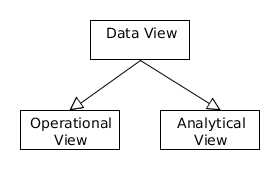
\includegraphics[natwidth=\textwidth]{figures/datamodelling/dataviews.png}
 \centering
 \label{fig:dataviews}
 \caption{Sicht auf Daten. Operational View als Informationsquelle für taktische und Analytical View als Informationsquelle für strategische Entscheidungen.}
\end{figure}

S\o rensen, Fountas und Nash stellen in \cite{jour:Sorensen2010} ein Modell für \textit{Farming Management Information System} kurz FMIS vor. Dies soll als Basis für Planungssysteme wie es aus anderen Branchen als ERP bekannt ist eingesetzt werden. S\o rensen beschreibt dies als drei aufeinander aufbauende Systeme, siehe auch \ref{fig:fmishierarchy}.

\begin{figure}[h]
 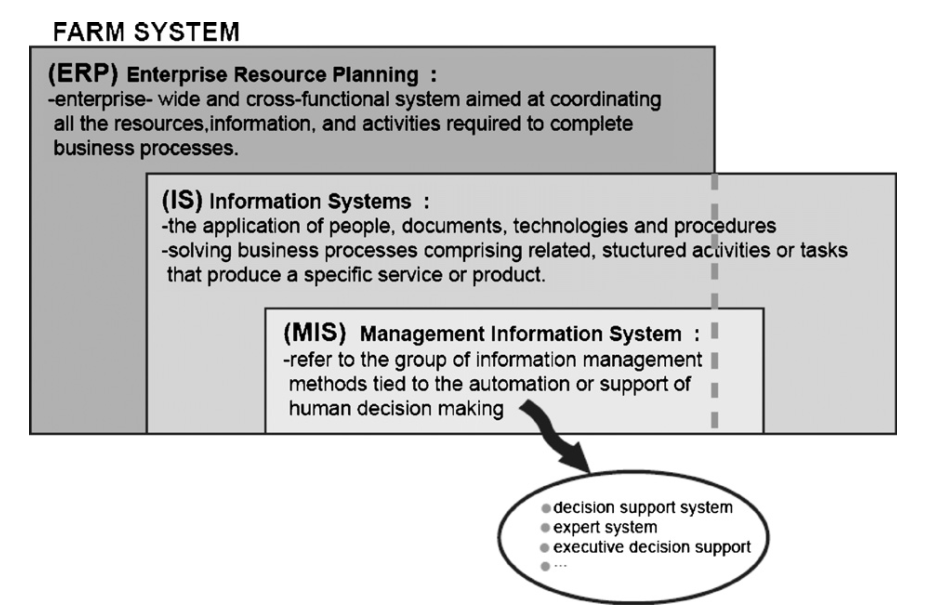
\includegraphics[scale=0.5,natwidth=\textwidth]{figures/datamodelling/sorensen_fmis_2010.png}
 \centering
 \label{fig:fmishierarchy}
 \caption{Konzept eines Management Information Systems.\cite{jour:Sorensen2010}}
\end{figure}

Neben diesen Sichtweisen die für die Entscheidungen im Betrieb wichtig sind, gehen Ruiz-Garcia, Steinberger und Rothmund in \cite{jour:Ruiz-Garcia2010} auf die Modellierung von Daten, Protokollen und Systemen ein, die es erlauben die Verarbeitung der Produkte in allen Schritten der Versorgungskette automatisch überwachen zu lassen. Dies dient dazu, den immer strenger werdenden gesetzlichen Bestimmungen (z.B. der ISO 22005 Standard zur Rückverfolgbarkeit der Lebensmittelbestandteile oder den EU Verordnungen Nr. 178/2002 bzw. Nr. 1935/2004) genügen zu können, ohne die Überprüfungen jedes Lieferanten manuell durchführen zu müssen.

\subsection{Operationale Sicht}
Die operationale Sicht dient dazu Entscheidungen in und für Geschäftsprozesse zu erleichtern bzw. zu ermöglichen. Unternehmerische Geschäftsprozesse werden in \cite{jour:Schulze2007} als Entscheidungen in einem begrenzten Zeitraum beschrieben. Dementsprechend ist es wichtig, dass die operationale Sicht vor allem Daten präsentiert die folgende Bedingungen erfüllen:

\begin{itemize}
	\item Die Daten müssen so aufbereitet werden, dass sie innerhalb der Prozesse verfügbar sind. (\textit{process-orientated data access})
	\item Die Daten müssen aktuell und detailliert sein.
	\item Die Daten müssen Zustände beschreiben. Zustände sollten lt. \cite{jour:Schulze2007} dabei als Menge von Attributen und Relationen zu anderen Zuständen definiert werden.
\end{itemize}

\subsection{Analytische Sicht}
Die analytische Sicht auf die bestehenden Daten leitet sich aus Messungen über einen bestimmten Zeitraum hinweg ab. Als Messungen sind Ergebnisse von bestimmten Berechnungen auf Klassifizierungspfade innerhalb der verfügbaren Datenbasis. In anderen Worten, geht es darum Aggregationen auf Relationen innerhalb von relevanten Ressourcen im Betrieb durchzuführen. Schulze macht dies am Beispiel eines Rinderzuchtsbetriebs für die Milchproduktion deutlich. Dabei werden Informationen über drei Ebenen hinweg aggregiert. So stellt die Sicht auf Ebene der Ställe andere Informationen als auf Ebene der einzelnen Kühe zur Verfügung. Siehe dazu Abbildung \ref{fig:kuehe}. 

\begin{figure}[h]
 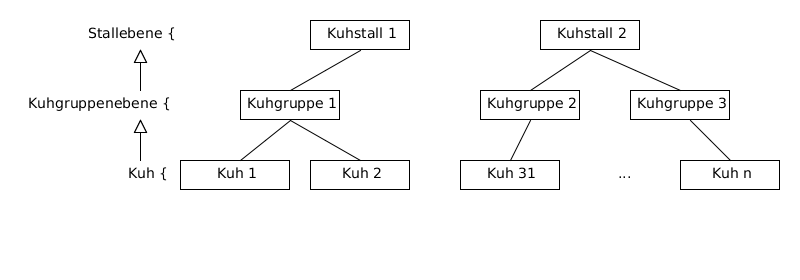
\includegraphics[scale=0.5,natwidth=\textwidth]{figures/datamodelling/kuehe.png}
 \centering
 \label{fig:kuehe}
 \caption{Klassifizierungsschema eines Milcherzeugungsbetriebs.}
\end{figure}

Dadurch wird die analytische Sicht im Unterschied zur operationalen Sicht, durch folgende Eigenschaften definiert:
\begin{itemize}
	\item Die analytische Sicht enthält auch historische Daten.
	\item Die analytische Sicht versucht verschiedene Datenquellen zu integrieren und ein Gesamtbild zu generieren.
	\item Die Daten werden ständig aggregiert und damit wiederverwendet.
\end{itemize}

Multidimensionale Daten können in Form von OLAP-Würfeln visualisiert werden.\ref{fig:kuehe_olap} 

\begin{figure}[h]
 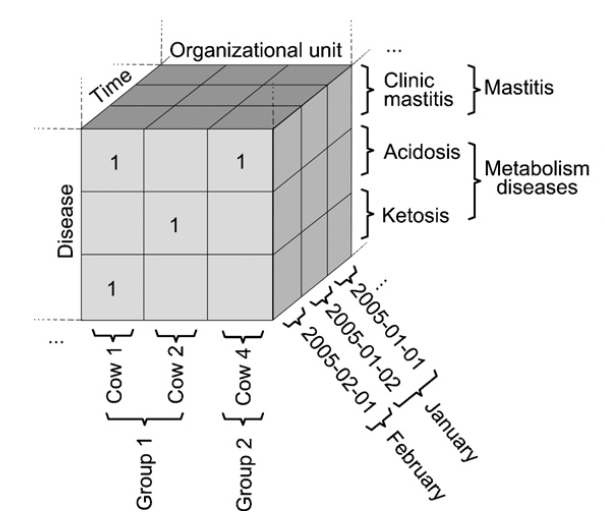
\includegraphics[scale=0.5,natwidth=\textwidth]{figures/datamodelling/kuehe_olap_wuerfel_schulze2007.png}
 \centering
 \label{fig:kuehe_olap}
 \caption{Darstellung der Daten eines Milcherzeugungsbetriebs in Form eines OLAP Würfelns.\cite{jour:Schulze2007}}
\end{figure}

Für die Speicherung und Verarbeitung von solch strukturierten Daten gibt es mehrere Ansätze. Die Daten können entweder getrennt gespeichert und verarbeitet werden in Form der Separierung in OLAP- und OLTP-System, oder auch zusammen geführt werden um die Auswertung auf aktuelleren Daten zu erlauben. Kemper stellt dafür in \cite{jour:Kemper2011} \textit{HyPer} vor.

\section{Entwurf von Datenmodellen}
Das Planen, Entwerfen und Erstellen von Datenmodellen ist ein Prozess, der im Zusammenspiel von Domänenexperten und Datenmodellierungsexperten durchgeführt werden muss. Sowohl S\o rensen wie auch Schulze schlagen dafür einen strukturierten Ansatz vor, der bei der Bestandsaufnahme der Akteure und Ressourcen beginnt und bei der Abbildung der verschiedenen Dimensionen und Relationen endet.\cite{jour:Schulze2007}\cite{jour:Sorensen2010}

Dem oder der Expertin für Datenmodellierung wird dabei nicht nur abverlangt die Relationen und Attribute in den verschiedenen Dimensionen formal abbilden zu können, sondern die Prozesse auch zu identifizieren um sie dann beschreiben zu können. Burkhart, Wolter, Schief, Di Valentin, Werth, Loos und Vaderhaeghen empfehlen dafür eine Ontologie zu entwerfen, stellten aber gleichzeitig fest, dass es noch keine Methode gibt, die völlig zufriedenstellend anleitet.\cite{jour:Burkhart2012} 

S\o rensen hat in \cite{jour:Sorensen2010} einen stark von der \textit{Soft Systems Methodology}, kurz SSM, beeinflussten Ansatz gewählt. SSM wurde entwickelt um praktische Erfahrungen systematisch in Erkenntnisse umzuwandeln. \cite{jour:Checkland2000}. Diese Erkenntnisse müssen in Prozessen abgebildet werden. In S\o rensens Versuch wurden in der Analysephase mit den Landwirten folgende Fragen geklärt:
\begin{itemize}
 \item Welche Akteure außerhalb des Betriebs müssen modelliert werden? (z.B. Behörden, Lieferanten, etc.)
 \item Welche Abläufe funktionieren gut im Betrieb? Wie funktionieren diese?
 \item Welche Abläufe funktionieren nicht zufriedenstellend? Wie funktionieren diese? Was würde der Landwirt bzw. die Landwirtin gerne daran ändern?
 \item Welche Informationen werden in der altäglichen Arbeit benötigt bzw. wie könnten diese aufbereitet werden um die Arbeit zu erleichtern?
\end{itemize}

Neben solchen Hardfacts sind auch Softfacts wichtig um während der Analyse ein möglichst vollständiges Bild (\textit{rich picture}) der abzubildenden Realität zu erhalten. Dementsprechend werden die Informationen aufgezeichnet um Beziehungen, Verbindungen, Einflüsse zwischen den verschiedenen Entitäten abzubilden.

Um aus diesen Informationen sinnvolle Prozesse und Informationsquellen ableiten zu können, müssen die richtigen Fragen gestellt werden. SSM stellt dafür eine Anleitung zur Verfügung der bei der Gestaltung helfen soll: \textit{CATWOE}. CATWOE ist eine Sammlung von Aspekten die beachtet werden müssen:
\begin{itemize}
	\item \textit{C} Customers. Wessen Problem soll gelöst werden?
	\item \textit{A} Actors. Wer sind die Akteure des Systems?
	\item \textit{T} Transformation Process. Dies definiert was das System ausführt, wie es die Eingabe- in Ausgabewerte umwandelt, wohin Ausgabewerte geschoben werden, welche Stadien und Schritte in diesem System existieren.
	\item \textit{W} World View. Die Weltanschauung definiert in welchem Kontext das System eingebettet ist. Was bedeutet es wenn das System ausgeführt wird? Was bedeutet eine Fehlfunktion oder ein Ausfall?
	\item \textit{O} Owners. Definiert Personen die, die formale Macht haben über Einführung oder Ablehnung des Systems haben.
	\item \textit{E} Environmental constraints. Definiert welche Grenzen dem System gesetzt sind, egal ob es sich dabei um ethische, juristische, personeller oder Grenzen anderer Natur handelt.
\end{itemize}

Schulz schlägt vor, zur Modellierung der Daten auf ein erweitertes \textit{Entity Relationship Modell}, kurz ER-Modell zurück zu greifen und hat dies auch exemplarisch vorgeführt. 


